%This is my super simple Real Analysis Homework template

\documentclass{article}
\usepackage[english]{babel}
\usepackage[]{amsthm} %lets us use \begin{proof}
\usepackage[]{amssymb} %gives us the character \varnothing
\usepackage{mathtools}
\usepackage{lineno}
\usepackage[ansinew]{inputenc}
\newcommand{\R}{\mathbb{R}}
\newcommand{\uproman}[1]{\uppercase\expandafter{\romannumeral#1}}
\title{Solutions Sheet 1}
\author{Yannick Zelle and Nina Fischer}
\date\today
%This information doesn't actually show up on your document unless you use the maketitle command below

\begin{document}
\maketitle %This command prints the title based on information entered above

%Section and subsection automatically number unless you put the asterisk next to them.


%Basically, you type whatever text you want and use the $ sign to enter "math mode".
%For fancy calligraphy letters, use \mathcal{}
%Special characters are their own commands

\section*{Exercise 1}
 First, we will assign values to $p(M), p(m), p(e), P(n\mid M), P(n\mid m), P(n\mid e)$, so that $p(M) + p(m) + p(e) = 1$:
 
 \[ p(M) := 0.01 \]
 \[ p(m) := 0.1 \]
 \[ p(e) := 0.89 \]
 
 \[ p(n\mid M)=0.9 \]
 \[ p(n\mid m)=0.08 \]
 \[ p(n\mid e)=0.02 \]
 
 The next step to apply Bayes' rule is now to calculate the probability of a noise:
 
 \[p(n)= p(M) \cdot p(n\mid M) + p(m) \cdot p(n\mid m) + p(e) \cdot p(n\mid e)\]
 
 \[ = 0.01 \cdot 0.9 + 0.1 \cdot 0.08 + 0.89 \cdot 0.02\]
 
 \[ = 0.0348\]
 
 We can now calculate the probability of a monster given noise by applying Bayes' rule:
 
 \[ p(M \mid n) =\frac{p(n \mid M) \cdot p(M)}{p(n)}
 \]
 \[=\frac{0.9 \cdot 0.01}{0.034} \]
 \[\approx 0.26\]
 
 These results got confirmed by the jupyter notebook presented in the lecture:
 
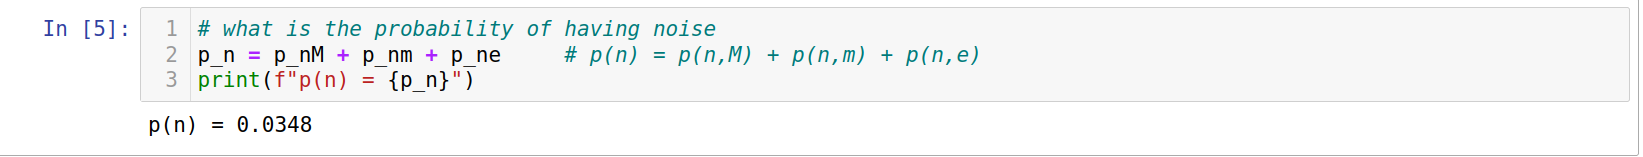
\includegraphics[width=10cm, height=1cm]{1}
\newline 
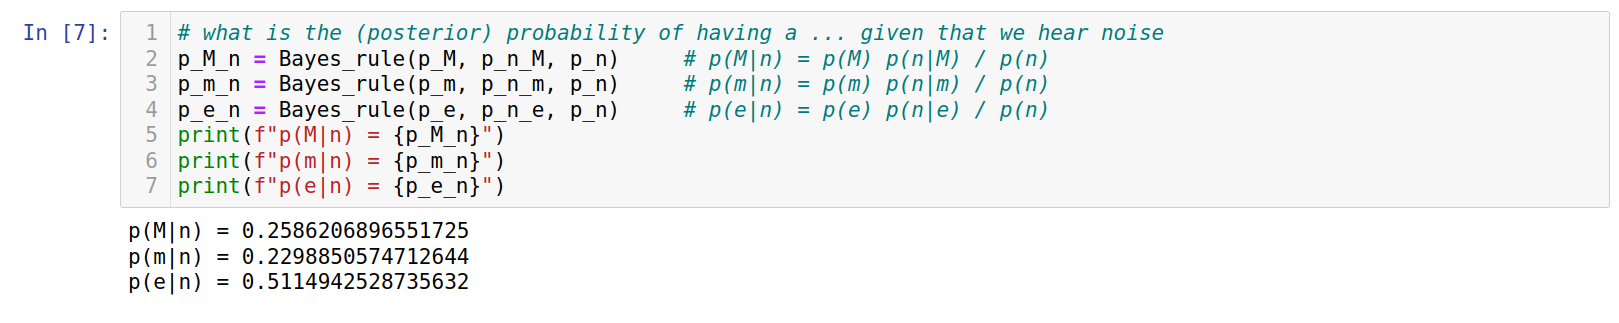
\includegraphics[width=10cm, height=2cm]{2}



\section*{Exercise 2}
\textbf{Given:} 
\begin{itemize}
\item The plausibility of $B$ is $p(B)$.
\item $p(B \mid A) \geq p(B)$
\end{itemize}

\textbf{Show:}
\textbf{(a)} $p(B \mid A) \geq p(B)$


\begin{proof}
Is equivalent to second assumption.
\end{proof}


\textbf{(b)} $p(B \mid \neg A) \leq p(B)$
\begin{proof}
By assumption:
\begin{align*}
& p(B|A) \geq p(B) \\
& \Leftrightarrow \frac{p(A \mid B) \cdot p(B)}{p(A)} \geq p(B)\\
& \Leftrightarrow \frac{(1-p(\neg A \mid B)) \cdot p(B)}{1-p(\neg A)} \geq p(B) \\
& \Leftrightarrow (1-p(\neg A \mid B)) \cdot p(B) \geq p(B)\cdot (1-p(\neg A)) \\
& \Leftrightarrow 1-p(\neg A \mid B)  \geq  1-p(\neg A) \\
& \Leftrightarrow -p(\neg A \mid B)  \geq  -p(\neg A) \\
& \Leftrightarrow p(\neg A \mid B)  \leq  p(\neg A) \\
& \Leftrightarrow p(\neg A \mid B)  \leq  p(\neg A)\cdot \frac{p(B)}{p(B)} \\
& \Leftrightarrow \frac{p(\neg A \mid B) \cdot p(B)}{p(\neg A)}  \leq  p(B) \\
& \Leftrightarrow p(B \mid \neg A)   \leq  p(B)
\end{align*}
\end{proof}



\textbf{(c)} $p(A \mid B) \geq p(A)$
\begin{proof}
By assumption:
\begin{align*}
& p(B|A) \geq p(B) \\
& \Leftrightarrow \frac{p(A \mid B) \cdot p(B)}{p(A)} \geq p(B)\\
& \Leftrightarrow p(A \mid B) \geq p(A) 
\end{align*}
\end{proof}

\textbf{(d)} $p(A \mid \neg B) \leq p(A)$
\begin{proof}
By assumption:
\begin{align*}
& p(B|A) \geq p(B) \\
& \overset{(c)}{\Leftrightarrow} p(A \mid B) \geq p(A)
\\
& \overset{(b)}{\Leftrightarrow} p(A \mid \neg B) \leq p(A)
\end{align*}
\end{proof}

\section*{Exercise 3}
 For this exercise we will formalise the given facts as follows:
 \begin{enumerate}
 \item $C = \text{"The Patient has Cancer"}$
 \item $R = \text{"A Patient's Mammogram is positive"}$
 \end{enumerate}
We can therefore deduct from the given facts:
\begin{enumerate}
 \item $P(C)= 0.008$
 \item $P(R \mid C) = 0.9$
 \item $P(R \mid \neg C) = 0.07$
 \item $P(\neg C)=1-P(C)= 0.992$
 \item $P(R)=P(C)\cdot P(R \mid C) + P(\neg C)\cdot P(R \mid \neg C) = 0.008 \cdot 0.9 + 0.992\cdot 0.07 = 0.08 $
 \end{enumerate}
Given these deductions, we can now calculate the adressed probability that a patient has breast cancer given a positive Mammogram $P(C \mid R)$ by applying Bayes' Rule:
\begin{align*}
& P(C \mid R) \\
& = \frac{P(R\mid C)\cdot P(C)}{P(R)} \\
& = \frac{0.9\cdot 0.008}{0.08}\\
& = 0.09
\end{align*}
 
\section*{Exercise 4}
For this exercise we will formulate the given facts as follows follows :

\begin{itemize}
\item $W_A = \text{"The warden announces A"}$
\item $W_B = \text{"The warden announces B"}$
\item $W_C = \text{"The warden announces C"}$

\item $A=\text{"A is pardonned"}$
\item $B=\text{"B is pardonned"}$
\item $C=\text{"C is pardonned"}$

\end{itemize}
Before any announcement is made by the warden we obviously have :

\[P(A) = P(B)= P(C) = \frac{1}{3} \]

No Matter what the warden will eather announce $A$ or $B$, which brings us to the conclusion:

\[P(A)= P(W_B \mid A) + P(W_C \mid A) =\frac{1}{3}\]

Because in this case the warden flips a coin we know:

\[ P(W_B \mid A)= P(W_C \mid A) = \frac{1}{6} \]

We know that $P(W_B\mid B) = 0$  and we can therefore also  deduct that :

\[ P(W_B)= P(A) \cdot P(W_B \mid A) + P(C) \cdot P(W_B\mid C) = \frac{1}{3}+\frac{1}{6}=\frac{1}{2}\]

Now we can apply Bayes' formula to calulate the updatet probability after the Warden's announcement:

\begin{align*}
 P(A \mid W_B)&=\frac{P(W_B \mid A)\cdot P(A)}{P(W_B)} \\
&= \frac{\frac{1}{6} \cdot \frac{1}{3} }{\frac{1}{2}} \\
&=\frac{1}{3} 
\end{align*}

We also now that $P( W_B\mid C)=1$ . It follows:

\begin{align*}
 P(C \mid W_B)&=\frac{P(W_B \mid C)\cdot P(C)}{P(W_B)} \\
&= \frac{1 \cdot \frac{1}{3} }{\frac{1}{2}} \\
&=\frac{2}{3} 
\end{align*}

Therefore C's argument is right.


\end{document}
